\documentclass{article}

%=====================================================================
%============================= packages ==============================

%\usepackage{geometry}
\usepackage{amsmath}
\usepackage{amssymb}
\usepackage{stmaryrd}
\usepackage{fancyhdr}
\usepackage{natbib}
\usepackage[normalem]{ulem}
\usepackage{examples-slim}
\usepackage{xcolor}
\usepackage{graphicx}
\usepackage{float}
\usepackage{multirow}
\usepackage{booktabs}
\usepackage{colortbl}
\usepackage{caption}
\usepackage{subcaption}
\definecolor{black}{rgb}{0,0,0}
\usepackage[colorlinks, linkcolor=black, urlcolor=black, citecolor=black]{hyperref}

\bibpunct[; ]{(}{)}{;}{a}{}{,}  % natbib citation style

%=====================================================================
%========================= cross-references ==========================

% Flexible sec/fig/tbl/def cross-refs.
\newcommand{\Secref}[1]{Section~\ref{#1}}
\newcommand{\secref}[1]{section~\ref{#1}}
\newcommand{\dashsecref}[2]{sections~\ref{#1}--\ref{#2}}

\newcommand{\Defref}[1]{Def.~\ref{#1}}
\newcommand{\defref}[1]{def.~\ref{#1}}
\newcommand{\Defrefc}[2]{\Defref{#1}, clause~\ref{#2}}
\newcommand{\defrefc}[2]{\defref{#1}, clause~\ref{#2}}

\newcommand{\Figref}[1]{Figure~\ref{#1}}
\newcommand{\figref}[1]{figure~\ref{#1}}
\newcommand{\dashfigref}[2]{figures~\ref{#1}--\ref{#2}}
\newcommand{\Tabref}[1]{Table~\ref{#1}}
\newcommand{\tabref}[1]{table~\ref{#1}}

% Examples:
\newcommand{\eg}[1]{(\ref{#1})}
\newcommand{\subeg}[2]{(\ref{#1}\ref{#2})}
\newcommand{\dblsubeg}[3]{(\ref{#1}\ref{#2},~\ref{#3})}
\newcommand{\dashsubeg}[3]{(\ref{#1}\ref{#2}--\ref{#3})}

% In-text citations
\newcommand{\posscitet}[1]{\citeauthor{#1}'s~(\citeyear{#1})}
\newcommand{\sposscitet}[1]{\citeauthor{#1}'~(\citeyear{#1})}
\newcommand{\possciteauthor}[1]{\citeauthor{#1}'s}
\newcommand{\spossciteauthor}[1]{\citeauthor{#1}'}
\newcommand{\pgposscitet}[2]{\citeauthor{#1}'s~(\citeyear{#1}:~#2)}
\newcommand{\secposscitet}[2]{\citeauthor{#1}'s~(\citeyear{#1}:~$\S$#2)}
\newcommand{\pgcitealt}[2]{\citealt{#1}:~#2}
\newcommand{\seccitealt}[2]{\citealt{#1}:~$\S$#2}
\newcommand{\pgcitep}[2]{(\citealt{#1}:~#2)}
\newcommand{\seccitep}[2]{(\citealt{#1}:~$\S$#2)}
\newcommand{\pgcitet}[2]{\citeauthor{#1}~(\citeyear{#1}:~#2)}
\newcommand{\seccitet}[2]{\citeauthor{#1}~(\citeyear{#1}:~$\S$#2)}

%=====================================================================
%============================ text styles ============================

\newcommand{\word}[1]{\emph{#1}}
\newcommand{\tech}[1]{\textbf{#1}}
\definecolor{maroon}{HTML}{990000}
\newcommand{\highlight}[1]{{\color{maroon}#1}}

%=====================================================================
%============================== judgments ============================

\newcommand{\bad}{\sqz{${}^\ast$}}
\newcommand{\freebad}{${}^\ast$}
\newcommand{\marked}{\sqz{${}^\#$}}
\newcommand{\freemarked}{${}^\#$}

%=====================================================================
%=============================== model ===============================


\newcommand{\tuple}[1]{\ensuremath{\left< #1 \right>}}
\newcommand{\set}[1]{\ensuremath{\left\{ #1 \right\}}}
\newcommand{\True}{\texttt{T}}
\newcommand{\False}{\texttt{F}}
\newcommand{\Reals}{\mathbb{R}}
\newcommand{\given}{\mid}
\newcommand{\Indicator}{\mathbb{I}}

\newcommand{\sem}[1]{\ensuremath{\llbracket#1\rrbracket}}
\newcommand{\States}{W}
\newcommand{\state}{w}
\newcommand{\Lex}{\mathcal{L}}
\newcommand{\LexStar}{\Lex^{\ast}}
\newcommand{\LexSet}{\mathbf{L}}
\newcommand{\Messages}{M}
\newcommand{\msg}{m}
\newcommand{\Costs}{C}
\newcommand{\Prior}{P}
\newcommand{\LexPrior}{P_{\LexSet}}

\newcommand{\listenerZero}{l_{0}}
\newcommand{\speakerOne}{s_{1}}
\newcommand{\listenerOne}{l_{1}}
\newcommand{\SpeakerK}[1][k]{S_{#1}}
\newcommand{\ListenerK}[1][k]{L_{#1}}

\newcommand{\nullmsg}{\mathbf{0}}

%=====================================================================
%============================ annotations ============================

\let\oldmarginpar\marginpar
\renewcommand{\marginpar}[1]{\oldmarginpar[\color{red}\raggedright\scriptsize #1]{\color{red}\raggedright\scriptsize #1}}

\newcommand{\textnote}[1]{{\color{red}#1}}

%=====================================================================
%============================== colors ===============================

\definecolor{lightgray}{HTML}{CCCCCC} 

\definecolor{highlightcolor}{HTML}{D95F02}
\definecolor{annotationcolor}{HTML}{777777} 
\definecolor{worldinfocolor}{HTML}{E7298A}
\definecolor{lexcolor}{HTML}{D95F02}
\definecolor{costcolor}{HTML}{A6761D}
\definecolor{defcolor}{HTML}{D95F02}
%\definecolor{hurfordcolor}{HTML}{00CC33}
\definecolor{hurfordcolor}{HTML}{1B9E77}
\newcommand{\hurford}[1]{{\relax\color{hurfordcolor}#1}}
\newcommand{\definitional}[1]{\relax{\color{defcolor}#1}}

\newcommand{\graycell}[1]{{\cellcolor[gray]{.8}#1}}

%=====================================================================
%============================== helpers ==============================

\newcommand{\porq}{p\,\word{or}\,q}
\newcommand{\pandq}{p\,\&\,q}

\newcommand{\disjlexicon}[2]{
  \left[
    \begin{array}[c]{l@{ \ \mapsto \ } l}
      \porq    & \set{#1} \\
      \pandq   & \set{#2} \\
      \nullmsg & \set{w_{1}, w_{2}, w_{3}} \\
    \end{array}
  \right]}

\newcommand{\listenerMatrix}[6]{
  \begin{array}[c]{l *{4}{r}}
    \toprule
    #1 & w_{1} & w_{2} & w_{3} \\
    \midrule
    p        & #2 \\
    q        & #3 \\              
    \pandq   & #4 \\
    \porq    & #5 \\
    \nullmsg & #6 \\
    \bottomrule
  \end{array}}

\newcommand{\speakerMatrix}[4]{
  \begin{array}[c]{r *{5}{r}}
    \toprule
    #1 & p & q & \pandq & \porq & \nullmsg \\
    \midrule
    w_{1} & #2 \\
    w_{2} & #3 \\ 
    w_{3} & #4 \\ 
    \bottomrule
  \end{array}}

\newcommand{\ListenerKMatrix}[4]{
  \begin{array}[c]{l *{3}{r}}
  \toprule
    #1 & w_{1} & w_{2} & w_{3} \\
    \midrule
    \LexStar  & #2 \\
    \Lex_{1}  & #3 \\
    \Lex_{2}  & #4 \\
    \bottomrule
  \end{array}}

\newcommand{\SpeakerKMatrix}[4]{
  \begin{array}[c]{l *{3}{r}}
    \toprule
    \Lex_{#1} & \porq & \pandq & \nullmsg \\
    \midrule
    w_{1}  & #2 \\
    w_{2}  & #3 \\
    w_{3}  & #4 \\
    \bottomrule
  \end{array}}

\newcommand{\smalldisjlex}[3]{
  \setlength{\arraycolsep}{1pt}
  \left[
    \begin{array}[c]{l@{ \ \mapsto \ }r@{, \ } l@{ \ \mapsto \ }r@{, \ } l@{ \ \mapsto \ }r}
      A & \set{#1} &
      B & \set{#2} &
      X & \set{#3}
    \end{array}
  \right]}

\newcommand{\smalldisjlexTargetDef}{\smalldisjlex{\definitional{\mathbf{w_{1}}}}{w_{2}}{\definitional{\mathbf{w_{1}}}}}

\newcommand{\smalldisjlexTargetHuford}{\smalldisjlex{\hurford{\mathbf{w_{1}}}}{w_{2}}{\hurford{\mathbf{w_{2}}}}}

\definecolor{highlightcolor}{HTML}{D95F02}
\definecolor{annotationcolor}{HTML}{777777} 
\definecolor{worldinfocolor}{HTML}{E7298A}
\definecolor{lexcolor}{HTML}{D95F02}
\definecolor{costcolor}{HTML}{A6761D}
\definecolor{defcolor}{HTML}{D95F02}
\definecolor{hurfordcolor}{HTML}{00CC33}
\newcommand{\hurford}[1]{{\relax\color{hurfordcolor}#1}}
\newcommand{\definitional}[1]{\relax{\color{defcolor}#1}}

\definecolor{lightgray}{HTML}{CCCCCC} 
%\renewcommand{\graycell}[1]{\colorbox{lightgray}{#1}}
\newcommand{\whitecell}[1]{\colorbox{white}{#1}}

\newcommand{\lismat}[4]{
  \setlength{\arraycolsep}{1pt}
  \begin{array}[c]{l *{3}{r}}
    \toprule
    #1 & w_{1} & w_{2} & w_{1}{\vee}w_{2} \\
    \midrule
    A & #2\\
    X & #3 \\
    A\,\word{or}\,X & #4 \\
    \bottomrule
  \end{array}}

\newcommand{\spkmat}[4]{
  \setlength{\arraycolsep}{1pt}
  \begin{array}[c]{l *{3}{r}}
    \toprule
    #1 & A & X & A\,\word{or}\,X \\
    \midrule
    w_{1} & #2\\
    w_{2} & #3 \\
    w_{1}{\vee}w_{2} & #4 \\
    \bottomrule      
  \end{array}}                   

\renewcommand{\disjlexicon}[2]{
  \renewcommand{\arraystretch}{1}
  \left[   
    \begin{array}[c]{l@{ \ \mapsto \ } l}
      p   & \set{#1} \\
      q  & \set{#2} \\
    \end{array}
  \right]}

\newcommand{\closurelex}[6][1]{
  \renewcommand{\arraystretch}{1}
  \begin{array}[c]{*{8}{r}}
    \toprule
    &w_{1}&w_{2}&w_{3}&w_{1}{\vee}w_{2}&w_{1}{\vee}w_{3}&w_{2}{\vee}w_{3}&w_{1}{\vee}w_{2}{\vee}w_{3}\\
    \midrule
    p      & #2 \\
    q      & #4 \\
    \pandq & #3 \\
    \porq  & #5 \\
    \nullmsg & #6 \\
    \bottomrule
  \end{array}}


\begin{document}

%%%%%%%%%%%%%%%%%%%%%%%%%%%%%%%%%%%%%%%%%%%%%%%%%%%%%%%%%%%%%%%%%%%%%%

\title{Negotiating lexical uncertainty and expertise with disjunctive utterances}
\author{Roger Levy and Christopher Potts}
\maketitle

%%%%%%%%%%%%%%%%%%%%%%%%%%%%%%%%%%%%%%%%%%%%%%%%%%%%%%%%%%%%%%%%%%%%%%

\section{Background, claims, and approach}\label{sec:introduction}

\begin{examples}

\item There are well-known communicative pressures on disjunctive
  phrases of the form \word{X or Y} to be construed so that the
  meanings of \word{X} and \word{Y} are disjoint.

\item \posscitet{Hurford:1974} generalization (HG) is a direct
  statement of the overall communicative pressure. It says that,
  subject to certain exceptions, \word{X or Y} is felicitous only if
  the meanings of \word{X} and \word{Y} are disjoint.

\item The most widely studied instance of this is that \word{X or Y}
  is generally taken to conversationally implicate that its
  conjunctive counterpart \word{X and Y} is pragmatically inaccessible
  (false, inappropriate, irrelevant, unknown to the speaker,
  etc.). The two disjuncts are thus presented as non-overlapping
  options.

\item However, there are two types of frequent and felicitous
  disjunctions that violate this preference: what we call
  \tech{subsumptive disjunctions} like \word{boat or canoe} and
  \tech{definitional disjunctions} like \word{wine lover or oenophile}
  \citep{Horn89,Rohdenburg:1985}.

\item Subsumptive disjunctions are more routine that HG would seem to
  suggest. We have collected a large corpus of counterexamples. A few:
  \word{canoe or boat}, \word{Paris or France}, \word{China or
    Beijing}, \word{writer or playwright}, \word{tired or exhausted}.
  They seem to be easy to find.  See also \citet{Chemla-HurfordCounts}
  for quantitative study of similar patterns.

\item The truth behind HG is that subsumptive examples reliably signal
  what we broadly refer to as \tech{exclusivizing}, in keeping with
  the intuition behind HG.  The examples seem to be motivated by a
  wide range of factors centering around the speaker's desire to
  highlight a subcategory.

\item Definitional disjunctions seem like maximal violations of HG,
  where the entailment runs both directions. However, such examples
  have different motivations than subsumptive ones. Such readings seem
  meta-linguistic, in that the speaker seems to be teaching the
  listener about a word meaning.

\item Summarizing the empirical picture, we find a tension. On the one
  hand, \word{X or Y} is typically construed (and intended) as
  involving semantically disjoint \word{X} and \word{Y}, and
  violations of this at the level of literal content give rise to rich
  conversational implicatures. On the other hand, disjunction can be
  used to signal that the speaker regards the two disjuncts as
  synonymous.

\item The puzzle deepens when we see that the empirical picture,
  including the definitional disjunction readings, is not a quirk of
  English that we could perhaps blame on a nonce ambiguity. We know it
  is attested in a wide range of typologically and geographically
  diverse languages. This suggests that the full range of readings
  derives from the literal semantics of disjunction and systematic
  pragmatic pressures.

\item We seek to capture the full range of behavior within a single
  recursive Bayesian model of pragmatic reasoning.  These models find
  their conceptual origins in \posscitet{Lewis69} work on signaling
  systems, and their technical details build on ideas from the
  iterated best response models of \citet{Jaeger:2007} and
  \citet{Franke09DISS}. They have been shown to achieve tight
  correlations with experimental data (e.g.,
  \citealt{Frank:Goodman:2012}) and to contribute to artificial agents
  that communicate effectively with each other to solve a
  collaborative task \citep{Vogel-etal:2013}.

\item The model's crucial components:

  \begin{examples}
  \item It lets speakers communicate, not just about the world, but
    also about the language \citep{Smith:Goodman:Frank:2013}. This
    allows us to probe for inferences about the lexicon that do not
    impact the overall denotation of the disjunctive phrase (crucial
    for exclusivization inferences).

  \item Following \citet{Bergen:Goodman:Levy:2012} and
    \citet{Smith:Goodman:Frank:2013}, the \textbf{lexical uncertainty}
    property of our model is that it allows a flexible relationship
    between an atomic expression's literal meaning and its
    context-specific refined meaning (e.g., the literal meaning of
    \word{boat} includes \word{canoe}, but one of its context-specific
    refinements might exclude it).
  % \item Refined meanings are preserved through semantic composition
  %   Speakers and listeners start with probability distributions over
  %   possible refinements of each literal meaning, and can coordinate
  %   on the refined meaning intended in a given utterance through
  %   pragmatic inference.  
  \end{examples}

\item Within this model, the different readings naturally emerge
  depending on specific contextual parameters relating to speaker
  expertise, listener malleability, and information contained in the
  common ground.

\end{examples}

%%%%%%%%%%%%%%%%%%%%%%%%%%%%%%%%%%%%%%%%%%%%%%%%%%%%%%%%%%%%%%%%%%%%%%

\section{A closer look at the phenomena}\label{sec:data}

%=====================================================================

\subsection{Subsumptive disjunctions}\label{sec:data:subsumptive}

\begin{examples}
\item\label{ourcorpus} Counterexamples to Hurford's constraint:
  \url{http://goo.gl/VAGqnB}

\item Here is a small sample of the cases provided at the above link:

  \begin{examples}
  \item Stop discrimination of an \highlight{applicant or person} due to their tattoos.
  \item Promptly report any \highlight{accident or occurrence}.
  \item The anchor will lie on the bottom and the \highlight{canoe or boat} will be held by the stream's current.
  \item I believe that music can \highlight{change or affect} your emotions.
  \item ``As an \highlight{actor or performer}, you are always worried about what the next job's going to be,'' Hensley says.
  \item Many state arbitration statutes contemplate motions to \highlight{correct or modify} being made to the tribunal directly.
  \item James Clifford (1992, 1997) is the writer most associated with making the connection between culture and \highlight{travel or movement}.
  \item Being a \highlight{captain or officer} is a privilege, and with that privilege comes great responsibility.
  \end{examples}

\item The dataset includes 86 cases where the left disjunct entails
  the right, and 75 in which the right entails the left. (These
  numbers need to be updated; we'll be adding more examples.)

\item We don't have a rigorous sampling procedure, so we are not sure
  we can probe this distribution for tendencies, but it does show that
  both directions are attested.

  \marginpar{We could consider doing something systematic with
    countries and their major cities using Google N-grams.}

\item The obstacles to a rigorous sampling procedure are numerous:   
  \begin{examples}
  \item The vast majority of noun pairs exclude each other.
  \item WordNet should allow exploration of hierarchically organized
    nouns, but its views of entailment and synonym tend to be too
    flexible.
  \item Judgments about entailment are inherently very messy --- this
    is intrinsic to the phenomena and to our model.
  \end{examples}

\item However, we can say that, for any two nouns $N_{1}$ and $N_{2}$
  one believes to be in an overlap or proper entailment relation, a
  Web search for ``$N_{1}$ or $N_{2}$'' will generally yield
  counterexamples, as will ``$N_{2}$ or $N_{1}$''.% We have checked
  % that all of the examples discussed in \citealt{Hurford:1974} and
  % \citealt{Singh:2008} are attested in fluent English text on the
  % Web. These are included in the corpus linked in \eg{ourcorpus}.
  %
  % We could do this, but I am not sure of the value. A lot of 
  % Singh's examples seem contrived, but for irrelevant reasons.

\item\label{exclusive} It is an important feature of these data that
  there is often considerable uncertainty about whether the two terms
  are truly in an entailment relation. For instance, where
  \subeg{exclusive}{franceorparis} leaves little room to negotiate the
  meaning of the terms in any clear sense,
  \subeg{exclusive}{churchorsynagogue} is much less clear: some
  speakers have firm judgments that \word{church} and \word{synagogue}
  exclude each other, but the many occurrences of ``synagogues and
  other churches'' in real text indicate that this is not a
  universally shared view of the lexicon.

  \begin{examples}
  \item\label{franceorparis} ``The nuptials will take place in either
    France or Paris.''
  \item\label{churchorsynagogue} ``In 1940, 37 percent of us had gone
    to a church or synagogue in the last week.''
  \end{examples}

\item And we should take care even with our assertion that
  \word{France} and \word{Paris} invariably stand in an entailment
  relation. In contexts where France is being construed in terms of
  its countryside, or Paris in terms of its particular urban charms,
  \word{France} could come to mean something more like `Paris outside
  of France'.

\item This lexical uncertainty motivates our own explanation for why
  speakers utter HG-violating disjunctions (as they clearly do; see
  \eg{ourcorpus}).

\item The examples seem to be motivated by a factors characterized in
  terms of the speaker's goal of ensuring that a specific subkind of
  the general term is included in the overall claim:

  \begin{examples}
  \item I(nformativeness)-implicature: when the listener might
    construe the general term as \emph{limited to} a salient or
    prototypical subkind. For example, where \word{boat} tends to
    identify motorboats, the speaker uses \word{boat or canoe} to
    ensure that canoes are included.
    
  \item Q(uantity)-implicature: where failure to explicitly mention a
    salient or prototypical subkind might trigger an ad-hoc scalar
    implicature of its \emph{exclusion} \citep{hirschberg:1985}. (The
    speaker uses \word{swimwear or bikini} to ensure that bikinis are
    included.)
  \end{examples}

\item Assume that $\sem{a} \subset \sem{A}$. Then, in both of the
  above cases, the speaker is concerned that $A$ will be construed as
  $\sem{A}-\sem{a}$, so using the disjunction ensures that the overall
  denotation of the disjunction is equivalent to $\sem{A}$ even if the
  listener in fact makes this assumption.

\item Anticipating our own explanation, we say that the speaker is
  hedging against the possibility that the listener's view of language
  is such that, at least in the current context, $\sem{A} \cap \sem{a}
  = \emptyset$, or perhaps, more weakly, $ \sem{a} \nsubseteq \sem{A}
  = \emptyset$. We think this is well-aligned with the guiding ideas
  of \citet{Chemla-HurfordCounts}.

\item An HG-violating disjunction like \word{boat or canoe} is more
  prolix than just \word{boat}, but the meaning of the disjunction
  includes \word{canoe} even if the listener interprets \word{boat}
  with a narrower refined meaning.  A speaker who places sufficiently
  high utility on conveying the broader meaning of \word{boat} will be
  willing to pay the cost of the additional disjunct to forestall
  misinterpretation.

\item The above observations extend to \posscitet{Singh:2008} proposed
  extension of HG to cases involving semantically overlapping
  disjuncts. It's very hard to make the relevant judgments.  If the
  sense of overlap is extensional, then even examples like
  \word{doctor or lawyer} will be counterexamples. If the sense of
  overlap is definitional, then it is extremely hard to figure out
  what criteria should be used to decide particular cases. 

\item However, our account does not require us to sort these issues
  out. Rather, it simply makes predictions about how lexical
  uncertainty will relate to potential lexical overlap between
  disjuncts. We are broadly in agreement with
  \citeauthor{Singh:2008}'s intuition that disjunctions tend to lead
  to lexical exclusivization inferences, where the disjuncts are in
  entailment or just overlap relations.
\end{examples}
 
%%%%%%%%%%%%%%%%%%%%%%%%%%%%%%%%%%%%%%%%%%%%%%%%%%%%%%%%%%%%%%%%%%%%%%

\subsection{Definitional disjunctions}\label{sec:data:definitional}

\begin{examples}
\item Attested in Chinese, Finnish, German, Hebrew, Ilokano, Japanese,
  Russian, and Tagalog. This suggests that the origins are rooted in
  the meaning of disjunction and general pragmatic forces working on
  that meaning.

\item Contextual requirements: 

  \begin{examples}
  \item The speaker is mutually and publicly known to be an expert in
    the relevant domain.

  \item The speaker is mutually and publicly known to believe the
    listener to be a non-expert in the relevant domain.

  \item The speaker is mutually and publically known to have an
    interest in conveying information about the language itself,
    even if this communicative inefficiency in terms of the 
    information conveyed about the world.
  \end{examples}

\item In some naturalistic uses, definitional disjunction is also seen
  when it is not common ground that the listener doesn't know the
  novel term, but rather when there is value for the speaker in
  demonstrating knowledge of the novel term's meaning.  We suggest
  that these uses are derivative of the core usage that we have
  presented a model of.

\item Overt signals: ad hoc prosody, italics, quotation marks. There is
  clearly great pressure to signal definitional readings, though it is
  not an absolute requirement.

\item There can be uncertainty about whether the listener should
  regard the disjunction as definitional. This can persist even when
  one of the words is unknown to the listener. In such cases, the
  disjunctive meaning is just extremely general and will not do
  justice to the speaker's intentions.

\item The definitional meaning is secondary to the central message ---
  a sort of side-effect of the main utterance. This contrasts with
  overt definitions like \word{oenophile means `wine-lover'} or
  \word{oenophile: wine-lover} (in a dictionary context). Our model
  captures this by characterizing the definitional effect as an
  inference about the lexicon, rather than about the information
  conveyed.
  
\item Alternative forms achieving the same thing: apposition
  \word{oenophile (`wine-lover')}. There might be others. Apposition
  would seem to have a conjunctive semantics (broadly speaking), so it
  is striking that there seem not to be definitional uses of
  conjunction itself.

\item Definitional readings need not be perfectly definitional in the
  sense of complete, pure synonymy. Indeed, it is likely that no
  definition achieves this ideal, especially if connotational meaning
  is included. (Examples: \word{internet or computer network}, and
  even our wine-lover example, where \word{oenophile} seems to elevate
  the concept to something more refined than \word{wine lover} picks
  out.)
\end{examples}

%%%%%%%%%%%%%%%%%%%%%%%%%%%%%%%%%%%%%%%%%%%%%%%%%%%%%%%%%%%%%%%%%%%%%%

\section{Model}\label{sec:model}

%=====================================================================

\subsection{Definition}\label{sec:definition}

\begin{examples}
\item Basic ingredients:
  \begin{examples}
  \item $\States$ is a set of states (worlds, referents, propositions, etc.).
  \item $\Messages$ is a set of messages with designated null message $\nullmsg$.
  \item $\Lex: \Messages \mapsto \wp(\States)$ is a semantic interpretation function. $\Lex'(\nullmsg) = \States$
  \item $\LexSet = \set{\Lex' : \Lex'(\nullmsg) = \States \text{ and } \forall \msg \in \Messages{-}\set{\nullmsg}, \Lex'(\msg) \subseteq \Lex(\msg)}$
  \item $\Prior : \States \mapsto [0,1]$ is a prior probability
    distribution over states.    
  \item $\Costs : \Messages \mapsto \Reals$ is a cost function on messages.
  \end{examples}

\item Agents
  \begin{examples}
  \item\label{l0}%
    $\listenerZero(\state \given \msg, \Lex) \propto
    \frac{\mathbb{I}(\state \in \Lex(\msg))}{|\Lex(\msg)|}
    \Prior(\state)$

  \item\label{s1}% 
    $\speakerOne(\msg \given \state, \Lex) \propto
    \exp
    \left(
      \log\left(\alpha\,\listenerZero(\state \given \msg, \Lex) \right)
      - 
      \gamma\,\Costs(\msg)
    \right)$
    
  \item\label{l1}% 
    $\listenerOne(\state \given \msg, \Lex) \propto 
    \speakerOne(\msg \given \state, \Lex)
    \Prior(\state)$

  \item\label{Lk}%
    \setlength{\arraycolsep}{2pt}%  
    $\mspace{-4mu}\begin{array}[t]{r c l}
      \ListenerK(\state, \Lex \given \msg) 
      &=&
      \sum_{\Lex \in \LexSet} \listenerOne(\state \given \msg, \Lex) \ListenerK(\Lex \given \msg) 
      \\[1ex]
      \ListenerK(\Lex \given \msg) 
      &\propto& 
      \Prior(\Lex) \sum_{\state\in\States} \SpeakerK(\msg \given \state)\Prior(\state)
    \end{array}$
    
  \item\label{Sk}%
    $\SpeakerK(\msg \given \state, \Lex) \propto 
    \exp
    \left(
      \log
      \left(\alpha\,\ListenerK[k-1](\state \given \msg, \Lex)\right)
      - 
      \beta \log\left(\ListenerK[k-1](\Lex\given\msg)\right)
      -
      \gamma\,\Costs(\msg)
    \right)$
  \end{examples}
\end{examples}

%=====================================================================

\subsection{Returning to simple state/message signaling}

\begin{examples}
\item\label{lisnorm} $\ListenerK(\state \given \msg)  = \sum_{\Lex \in \LexSet} \ListenerK(\state, \Lex \given \msg)$
\item\label{spknorm} $\SpeakerK(\msg \given \state) \propto \sum_{\Lex \in \LexSet} \SpeakerK(\msg \given \state, \Lex)$
\end{examples}

%=====================================================================

\subsection{Illustrative examples}\label{sec:illustrations}

\begin{examples}
\item These initial examples are meant to show how the model works.
  They have been done elsewhere, but it seems worth reviewing them
  using our full model to ensure that the results are preserved.

% \item Because closure under disjunction is crucial to our analysis, we
%   do this for all our examples. (This is another respect in which we
%   are doing more than just repeating examples that have been done in
%   other papers.) 
%%
%%   We could see this through, but it's hard to make sense of it for
%%   the Manner case.
\end{examples}

%=====================================================================

\subsubsection{Scalar implicature}\label{sec:scalar}

\newcommand{\scalarstate}[1]{w_{#1}}
\newcommand{\wALL}{\scalarstate{\forall}}
\newcommand{\wSOMENOTALL}{\scalarstate{\exists\neg\forall}}

\newcommand{\scalarmsg}[1]{\text{#1}}
\newcommand{\mAll}{\scalarmsg{all}}
\newcommand{\mSome}{\scalarmsg{some}}
\newcommand{\mSomevAll}{\scalarmsg{some or all}}

\newcommand{\scalarlex}[3]{
  \left[
    \begin{array}[c]{l@{ \ \mapsto \ } l}
      \mAll & \set{#1} \\
      \mSome & \set{#2} \\
      \mSomevAll & \set{#3} \\
    \end{array}
  \right]}

\begin{examples}
\item
  \begin{examples}
  \item $\States = \set{\wALL, \wSOMENOTALL}$; $\Messages = \set{\mAll, \mSome}$
  \item $\Lex = [\mAll \mapsto \set{\wALL}, \mSome \mapsto \set{\wALL,\wSOMENOTALL}]$
  \item Flat prior; all $0$ costs; disjunction cost $0.1$; $\alpha = 1$; $\beta = 1$; $\gamma = 1$  
  \item Lexica with disjunctive closure of states and messages:
    \setlength{\arraycolsep}{2pt}
    \[
    \scalarlex{\wALL}{\wSOMENOTALL,\wALL}{\wSOMENOTALL, \wALL}
    \hfill
    \scalarlex{\wALL}{\wALL}{\wALL}
    \hfill
    \scalarlex{\wALL}{\wSOMENOTALL}{\wSOMENOTALL, \wALL} 
    \]
  \end{examples}
\end{examples}

\begin{examples}
\item $\ListenerK[3]$ after marginalization over lexica as in \eg{lisnorm} \\[-0.25ex]
  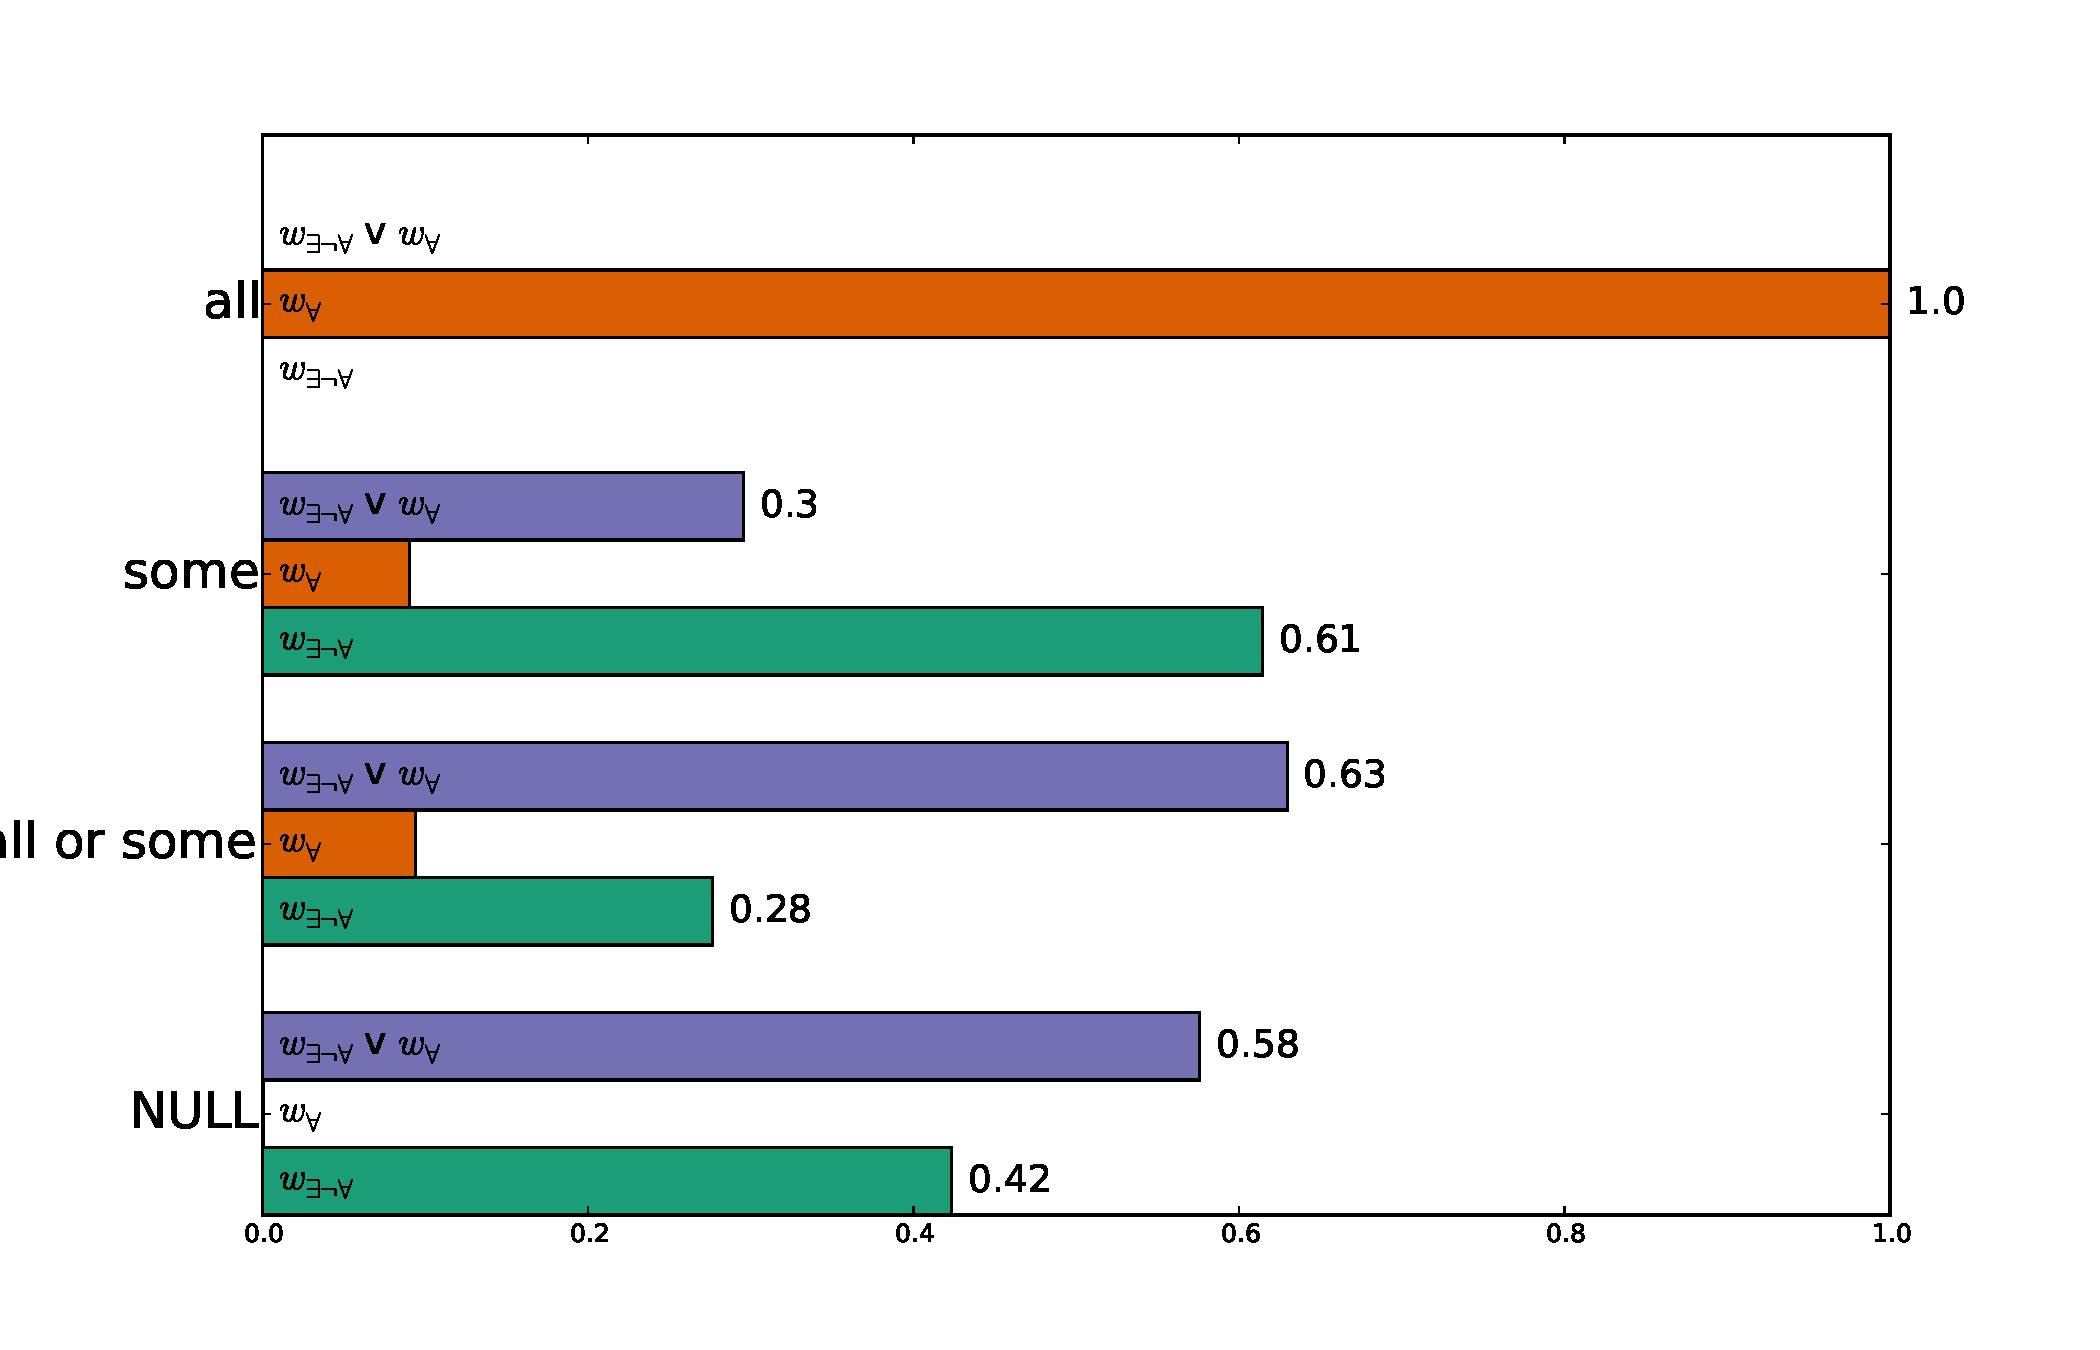
\includegraphics[width=0.6\textwidth]{fig/scalar-expertise-listener-marginalized}

\item $\SpeakerK[3]$'s message behavior given state--lexicon pairs:

  \vspace{-4pt}

  $\mspace{-140mu}$
  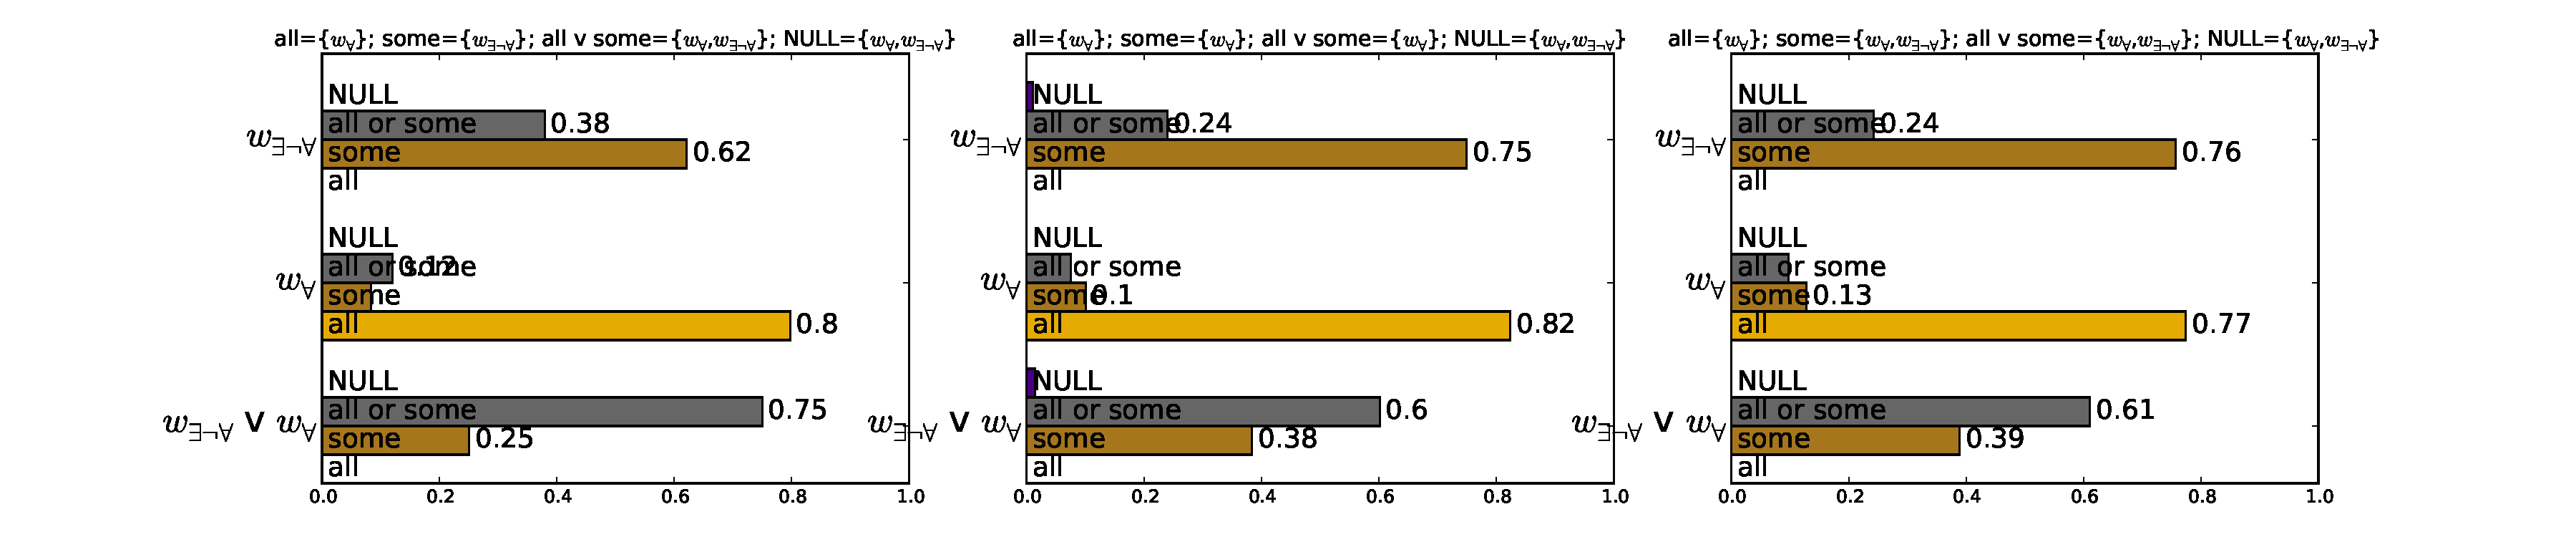
\includegraphics[width=1.4\textwidth]{fig/scalar-expertise-speaker}

\item $\SpeakerK[3]$ summed over lexica and renormalized as in \eg{spknorm} \\[-0.25ex]
  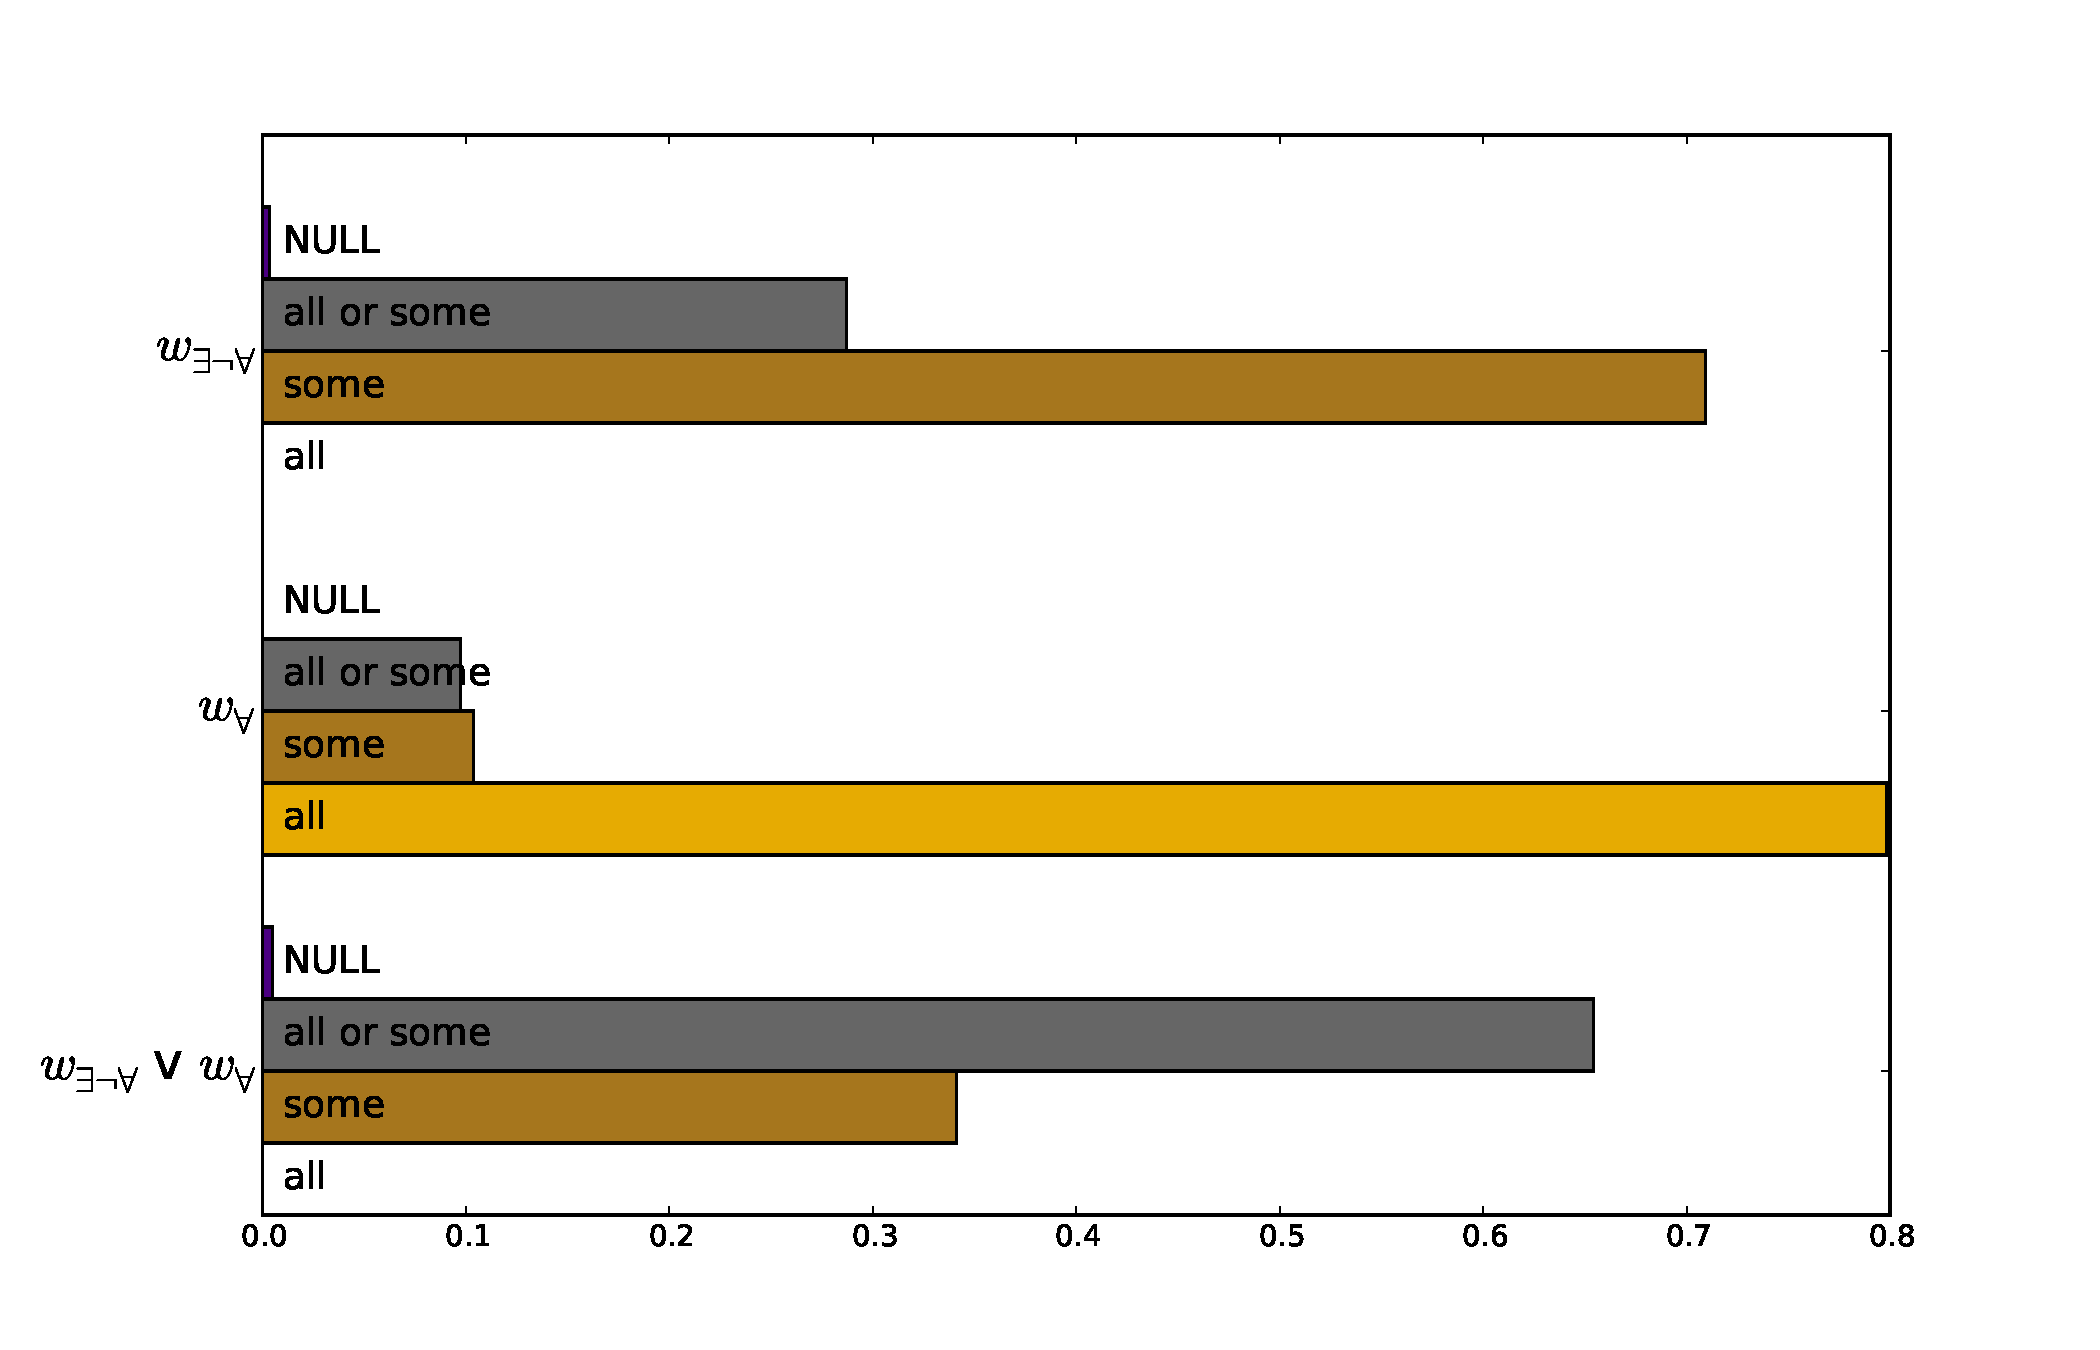
\includegraphics[width=0.6\textwidth]{fig/scalar-expertise-speaker-lexsum}
\end{examples}

%=====================================================================

\subsubsection{Markedness implicature}\label{sec:markedness}

\newcommand{\mSHORT}{\text{SHORT}}
\newcommand{\mLONG}{\text{long}}

\newcommand{\mannerstate}[1]{w_{\textsc{#1}}}
\newcommand{\wFREQ}{\mannerstate{freq}}
\newcommand{\wRARE}{\mannerstate{rare}}


\newcommand{\mannerlex}[2]{
  \left[
    \begin{array}[c]{l@{ \ \mapsto \ } l}
      \mSHORT & \set{#1} \\
      \mLONG & \set{#2}
    \end{array}
  \right]}

\begin{examples}
\item 
  \begin{examples}
  \item $\States = \set{\wFREQ,\wRARE}$ 
  \item $\Messages = \set{\mSHORT, \mLONG}$
  \item $\Lex = [\mSHORT \mapsto \set{\wFREQ,\wRARE}, \mLONG \mapsto \set{\wFREQ,\wRARE}]$
  \item $\Prior = [\wFREQ \mapsto 2/3, \wRARE \mapsto 1/3]$
  \item $\Costs = [\mSHORT \mapsto 1, \mLONG \mapsto 2]$
  \item $\alpha = 3$; $\beta = 1$; $\gamma = 1$  
  \item Lexica:
    \[
    \setlength{\arraycolsep}{2pt} 
    \begin{array}[c]{l l l}
      \mannerlex{\wFREQ,\wRARE}{\wFREQ,\wRARE}
      &
      \mannerlex{\wFREQ,\wRARE}{\wFREQ}
      &
      \mannerlex{\wFREQ,\wRARE}{\wRARE}
      \\[4ex]
      \mannerlex{\wFREQ}{\wFREQ,\wRARE}
      &
      \mannerlex{\wFREQ}{\wFREQ}
      &
      \mannerlex{\wFREQ}{\wRARE}
      \\[4ex]
      \mannerlex{\wRARE}{\wFREQ,\wRARE}
      &
      \mannerlex{\wRARE}{\wFREQ}
      &
      \mannerlex{\wRARE}{\wRARE}
    \end{array}
    \]
  \end{examples}
\end{examples}

\begin{examples}
\item $\ListenerK[3]$ after marginalization over lexica as in \eg{lisnorm} \\
  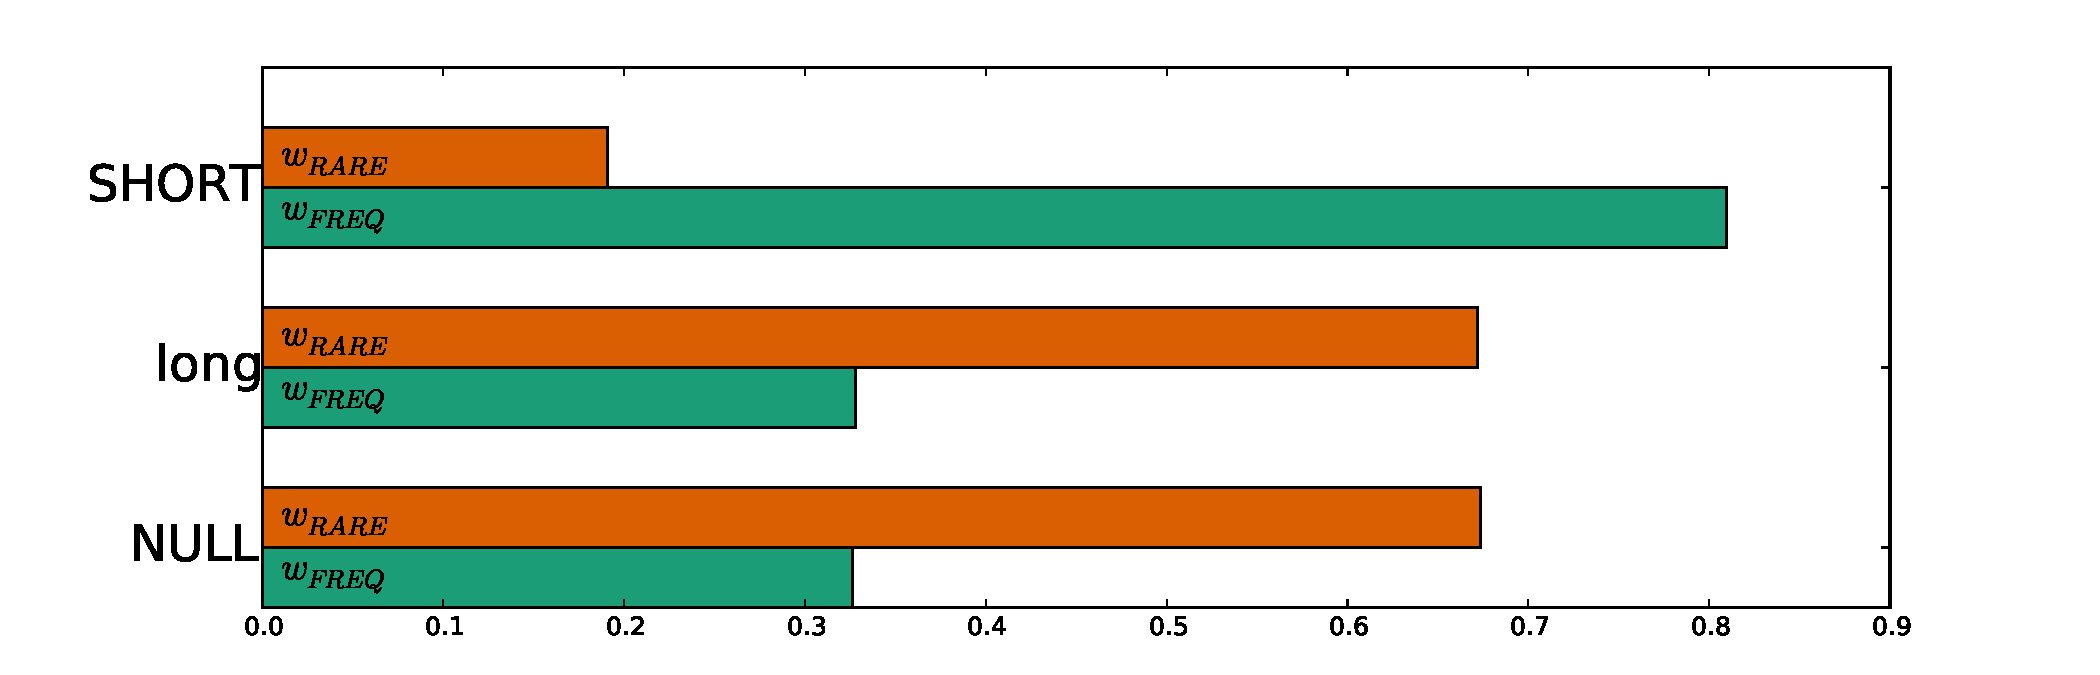
\includegraphics[width=0.7\textwidth]{fig/manner-expertise-listener-marginalized}

\item $\SpeakerK[3]$ summed over lexica and renormalized as in \eg{spknorm} \\
  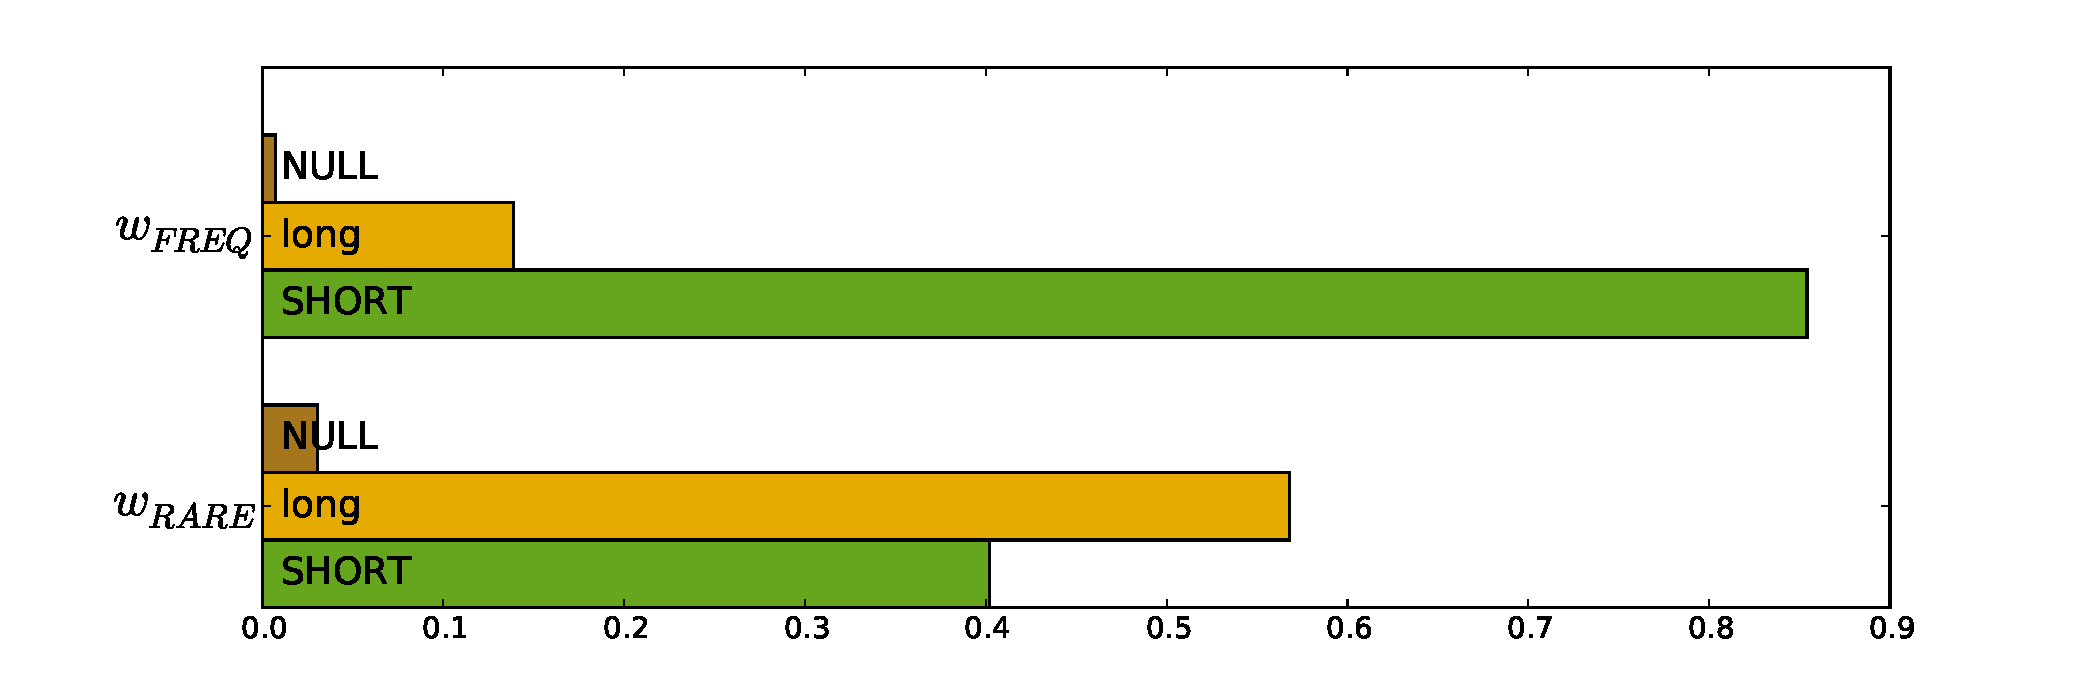
\includegraphics[width=0.7\textwidth]{fig/manner-expertise-speaker-lexsum}
\end{examples}

%=====================================================================
\newpage

\subsubsection{Scalar implicature of disjunction}\label{sec:scalar-disj}

\marginpar{We should talk about running this with meet joins. It seems more
  appropriate but it poses some challenges.}

\begin{examples}
\item 
  \begin{examples}
  \item 
    $\Lex$:
    $\begin{array}[c]{r *{4}{c}}
      \toprule
                    & p      & q      & p \word{ or } q & p \word{ and } q \\
      \midrule
      w_{1}          & \True    & \False & \True     & \False \\
      w_{2}          & \True    & \True  & \True     & \True  \\
      w_{3}           & \False  & \True  & \True     & \False \\
      \bottomrule
    \end{array}$
  \item $\alpha = 3$ (it's important that this be high for exclusivization)
  \item Disjunction cost: $0.1$; $\beta = 1$; $\gamma = 1$  
  \end{examples}
\end{examples}

\noindent
\begin{minipage}[c]{0.48\linewidth}
  \begin{examples}
  \item $\ListenerK[3]$ after marginalization 
    
    \vspace{-4pt}

     $\mspace{-90mu}$
     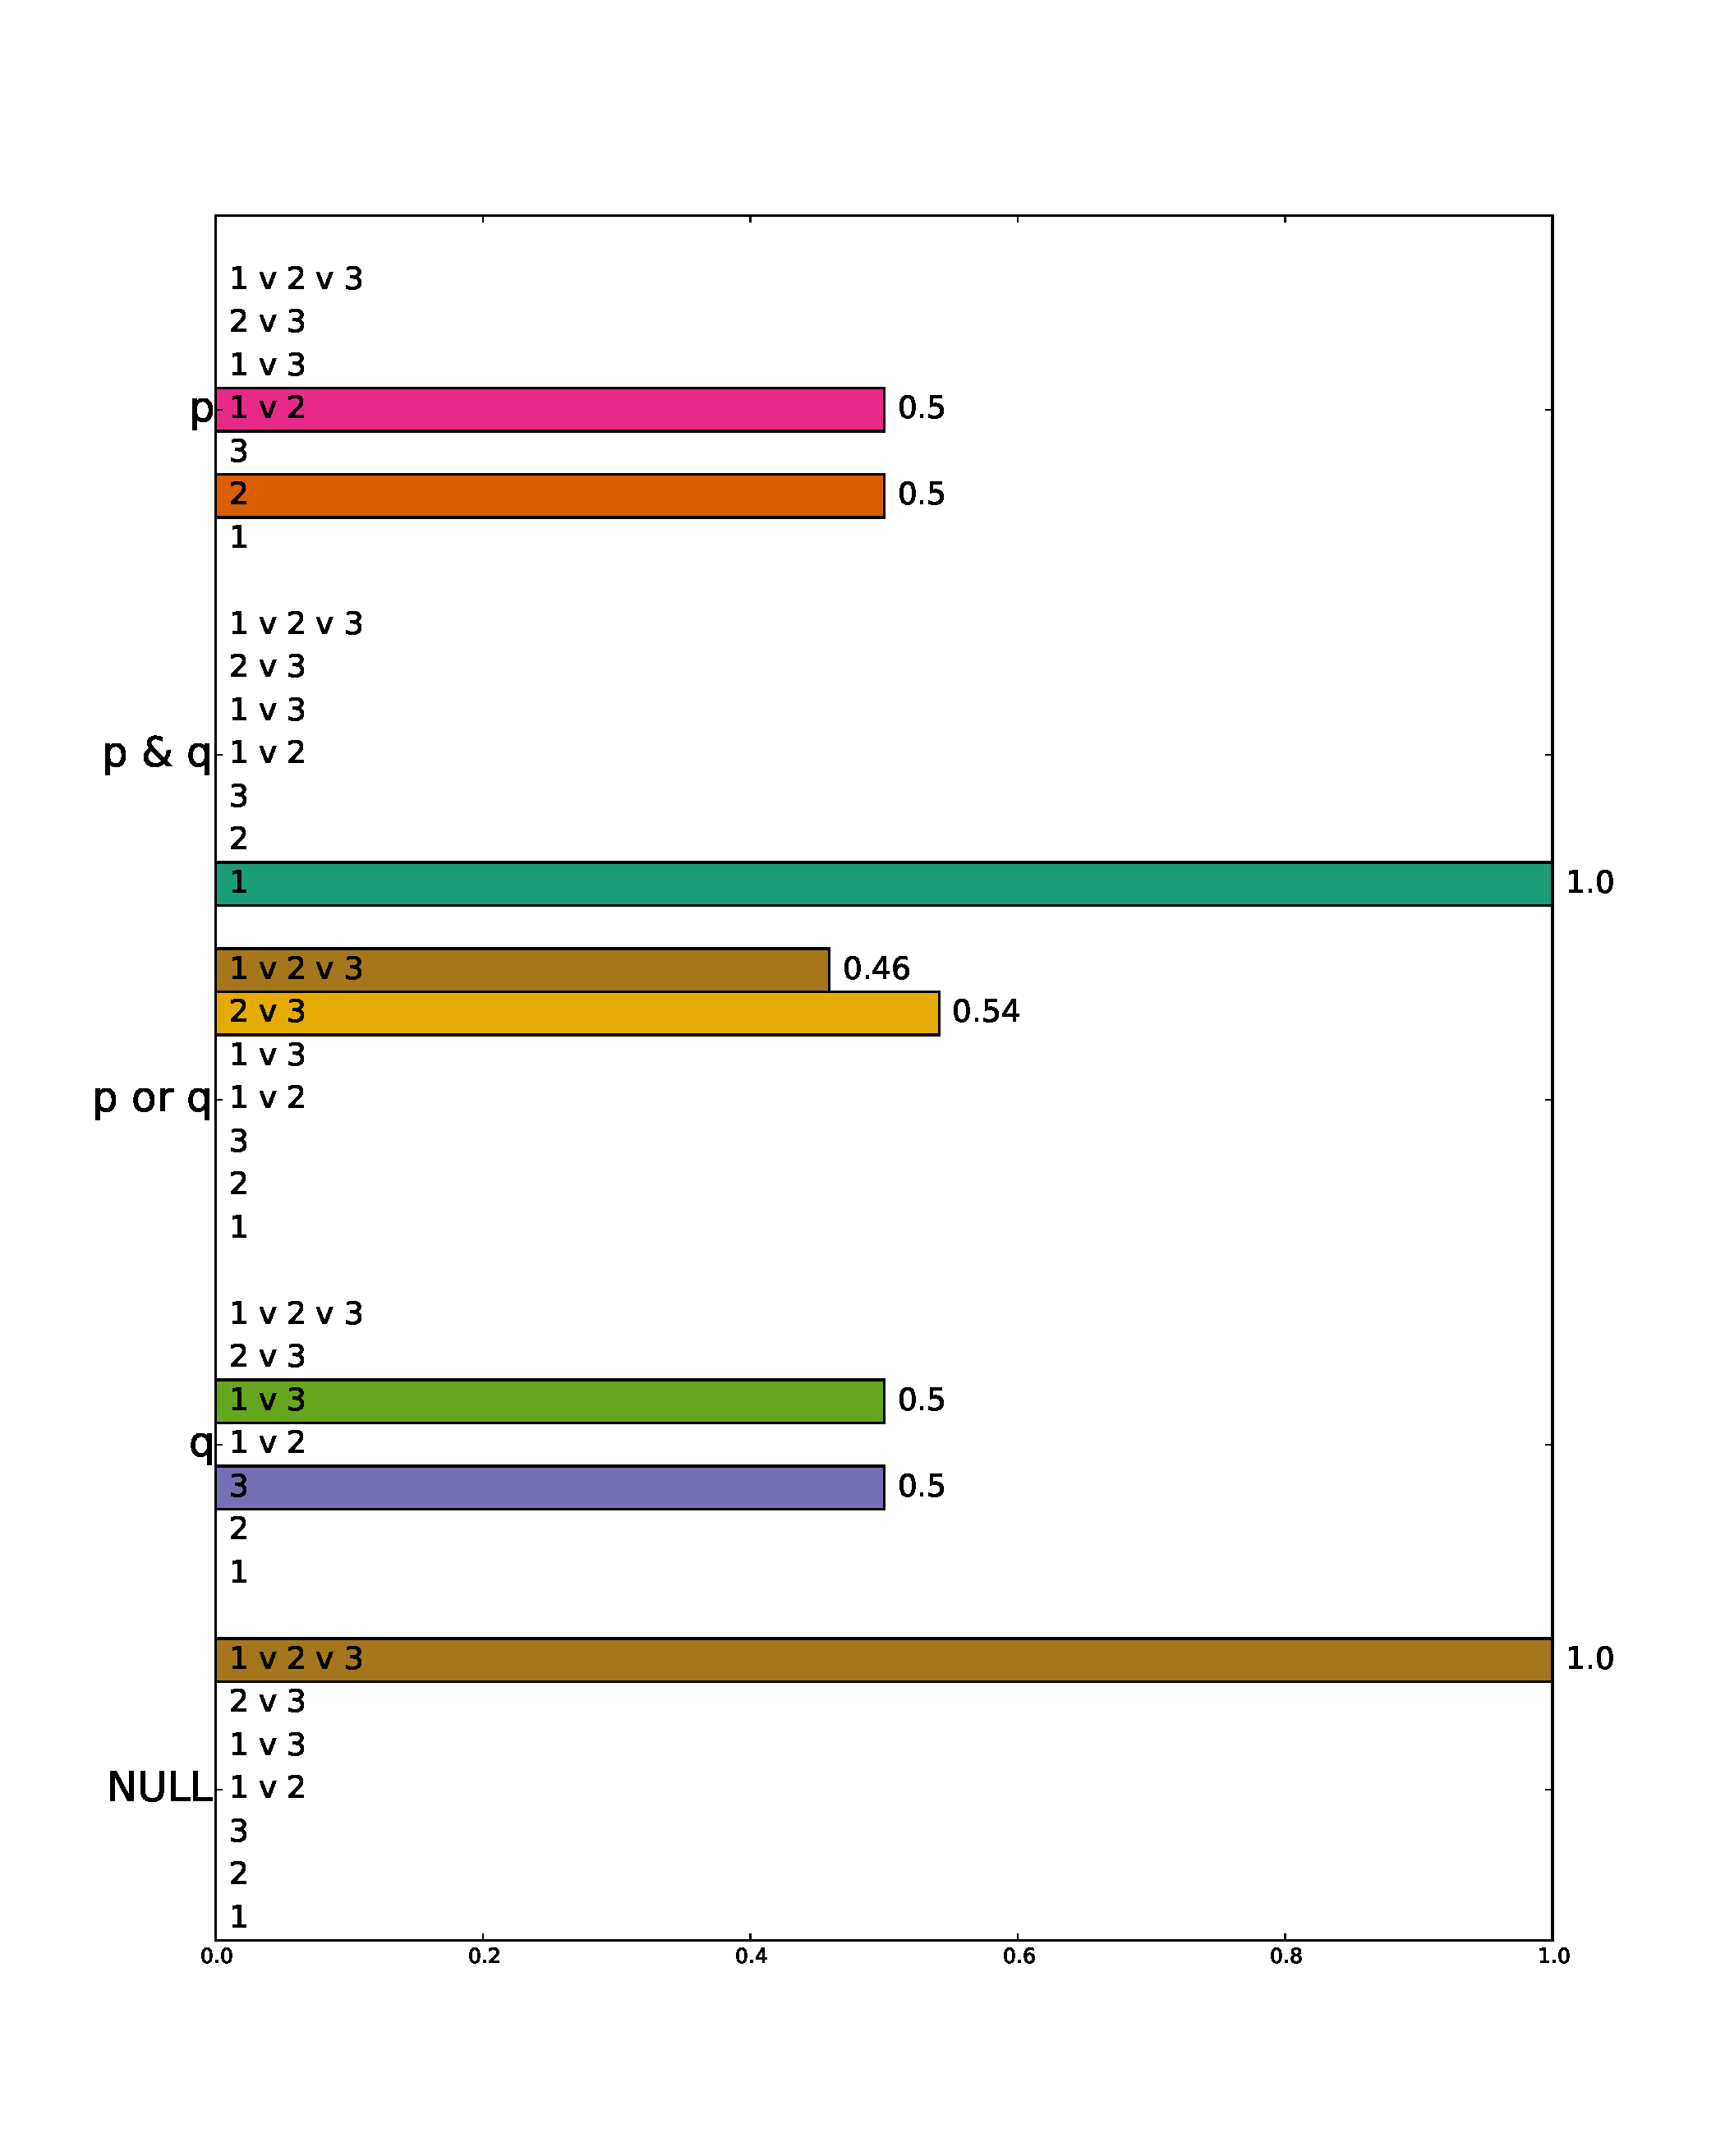
\includegraphics[width=1.2\textwidth]{fig/scalardisj-expertise-listener-marginalized}
  \end{examples}
\end{minipage}
\hfill
\begin{minipage}[c]{0.48\linewidth}
  \begin{examples}
  \item $\SpeakerK[3]$ summed over lexica
    
    \vspace{-4pt}

    $\mspace{-70mu}$
    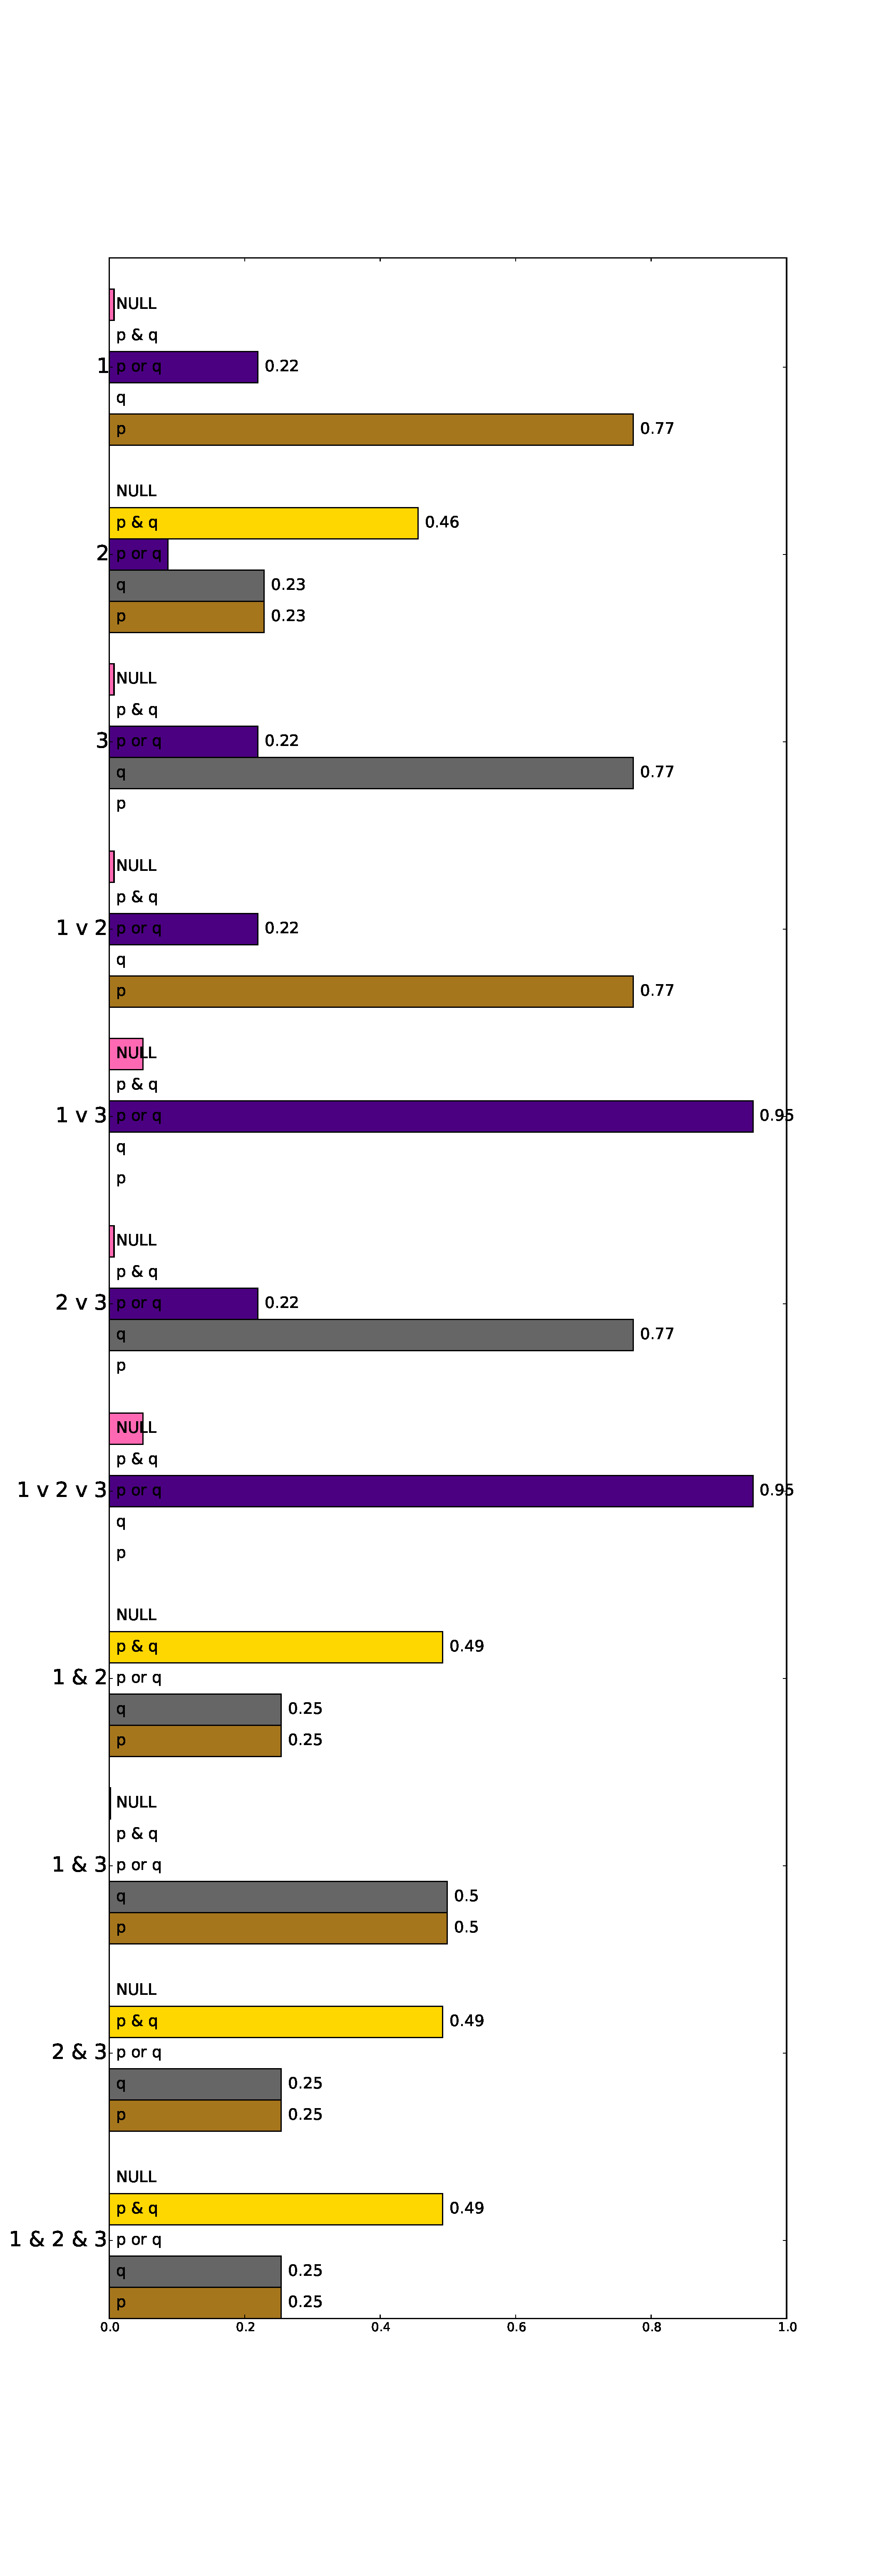
\includegraphics[width=1.2\textwidth]{fig/scalardisj-expertise-speaker-lexsum}
  \end{examples}
\end{minipage}

\begin{examples}
\item Summary of the above via max associations:

  \begin{minipage}[t]{0.45\linewidth}
    Listener

    \vspace{-2pt}
  
    $\begin{array}[t]{r @{ \ \Rightarrow \ } l}
      \toprule
      \text{Message} & \text{Inference} \\
      \midrule
      p &  w_{1}\\
      q & w_{3} \\
      p \word{ or } q & w_{1} \vee w_{3} \\
      \bottomrule
    \end{array}$
  \end{minipage}
  \hfill
  \begin{minipage}[t]{0.45\linewidth}
    Speaker

    \vspace{-2pt}

    $\begin{array}[t]{r @{ \ \Rightarrow \ } l}
      \toprule
      \text{Observation} & \text{Best message} \\
      \midrule
      w_{1} & p \\
      w_{2} & \set{p, q} \\
      w_{3} & q  \\      
      w_{1} \vee w_{3} & p \word{ or } q \\
      \bottomrule
    \end{array}$
  \end{minipage}    
\end{examples}

%=====================================================================

\section{Analysis}\label{sec:analysis}

\begin{examples}
\item Throughout, let \word{X} be the unknown term.

\item From the listener's perspective, we are concerned to see when
  \word{A or X} gives rise to the inference that $\sem{A} \cap \sem{X}
  = \emptyset$ (Hurfordian reading) and when \word{A or X} gives rise
  to the inference that $\sem{A} = \sem{X}$ (definitional).
\end{examples}

\newcommand{\smallhurfordlex}[3]{
  \left[
    \begin{array}[c]{l@{ \ \mapsto \ }r l@{ \ \mapsto \ }r l@{ \ \mapsto \ }r}
      A & \set{#1} &
      B & \set{#2} &
      X & \set{#3}
    \end{array}
  \right]}

%=====================================================================

\subsection{Subsumptive disjunctions}\label{sec:analysis:subsumptive}

\begin{examples}
\item From the listener's perspective, we are concerned to see when
  \word{A or X} gives rise to the lexical inference that $\sem{A} \cap
  \sem{X} = \emptyset$. We assume that the overall meaning will be
  $\sem{A} \cup \sem{X}$, i.e., that the relevant information concerns
  just the lexical inference.

\item Here's a scenario in which the exclusivization inference arises:

  \begin{examples}
  \item $\States = \set{w_{1}, w_{2}, w_{3}}$;  $\Messages = \set{A, B, X}$
  \item $\Lex = [A \mapsto \set{w_{1}}, B \mapsto \set{w_{2}}, X \mapsto \set{w_{1}, w_{2}}]$
  \item Priors are flat. $\alpha = 2$; $\beta = 1$; $\gamma = 1$. Disjunction cost: $1$. $n = 3$. 
  \end{examples}

\item The listener's best guess inference, upon hearing \word{A or X},
  is that the speaker's state is $w_{1} \vee w_{2}$ and that the
  lexicon is the one where $A$ and $X$ are disjoint. Here's the joint
  probability table:
  \[
  \renewcommand{\arraystretch}{2}
  \begin{array}[c]{l r r r}
    \toprule
            & w_{1} & w_{2} & w_{1} \vee w_{2} \\
    \midrule
    \smallhurfordlex{w_{1}}{w_{2}}{w_{1}, w_{2}} & 0 & 0 & 0.16 \\
    \smallhurfordlex{w_{1}}{w_{2}}{w_{2}} & 0 & 0 & \graycell{0.47} \\
    \smallhurfordlex{w_{1}}{w_{2}}{w_{1}} & 0 & 0 & 0.38 \\
    \bottomrule
  \end{array}
  \]

\item The above parameters deliver the same result with the the
  lexicon size increased (same pattern: each lexical item denotes its
  own world and $X$ denotes the union of all the worlds). This is
  unwieldy to visualize, but the important thing is that the best
  lexicon is always a Hurfordian one. Here's the best lexical
  inference with five atomic messages and four atomic states:
  \[
  \left[
    \begin{array}[c]{l@{ \ \mapsto \ }l}
      A & \set{w_{1}} \\
      B & \set{w_{2}} \\
      C & \set{w_{3}} \\
      D & \set{w_{4}} \\
      X & \set{w_{2}, w_{3}, w_{4}}
    \end{array}
  \right]
  \]
  This is the `minimal' Hurfordian lexicon: the listener doesn't infer
  anything about $X$ except that it is disjoint from $A$.    
\end{examples}

%=====================================================================

\subsection{Definitional disjunctions}\label{sec:analysis:definitional}

\begin{examples}
\item From the listener's perspective, we are concerned to see when
  \word{A or X} is interpreted as equivalent to $\sem{A}$.

\item From the speaker's perspective, we want to know what happens
  when the speaker favors a lexicon in which $\sem{A}=\sem{X}$ and
  observes a state equivalent to the literal meaning of $\sem{A}$.
  When will such a speaker produce \word{A or X}.

\item Here's an example in which these two perspectives are
  complementary. To achieve it, we have to substantially raise
  $\alpha$ and $\beta$ and lower disjunction costs:

  \begin{examples}
  \item $\States = \set{w_{1}, w_{2}, w_{3}}$;  $\Messages = \set{A, B, X}$
  \item $\Lex = [A \mapsto \set{w_{1}}, B \mapsto \set{w_{2}}, X \mapsto \set{w_{1}, w_{2}}]$
  \item Priors are flat. $\alpha = 5$; $\beta = 7$; $\gamma = 1$. Disjunction cost: $0.01$. $n = 3$. 
  \end{examples}

\item The listener's best guess inference, upon hearing \word{A or X},
  is that the speaker's state is $w_{1} \vee w_{2}$ and that the
  lexicon is $\Lex_{1}$. Here's the joint probability table:
  \[
  \renewcommand{\arraystretch}{2}
  \begin{array}[c]{l r r r}
    \toprule
            & w_{1} & w_{2} & w_{1} \vee w_{2} \\
    \midrule
    \smallhurfordlex{w_{1}}{w_{2}}{w_{1}, w_{2}} & 0 & 0 & 0 \\
    \smallhurfordlex{w_{1}}{w_{2}}{w_{2}}        & 0 & 0 & 0 \\
    \smallhurfordlex{w_{1}}{w_{2}}{w_{1}}        & \graycell{0.88} & 0 & 0.12\\
    \bottomrule
  \end{array}
  \]

\item The above parameters deliver the same result with the the
  lexicon size increased. Here's the best lexical inference with five
  atomic messages and four atomic states --- in this way, the 
  listener has learned that $A$ and $X$ are synonymous:
  \[
  \left[
    \begin{array}[c]{l@{ \ \mapsto \ }l}
      A & \set{w_{1}} \\
      B & \set{w_{2}} \\
      C & \set{w_{3}} \\
      D & \set{w_{4}} \\
      X & \set{w_{1}}
    \end{array}
  \right]
  \]  

\item If we assume that the unknown term has an atomic meaning, then
  we can strengthen the inference (and generate it under a wider range
  of parameters settings).  Under these circumstances, the meaning of
  the known disjunct serves as a \emph{focal point} that the speaker
  and listener can coordinate on for the meaning of the unknown word.
\end{examples}

%=====================================================================

\subsection{Characterization}\label{sec:analysis:characterization}

\begin{examples}
\item The basic characterization is that definitional reading arise
  when disjunction costs are low and $\beta$ is high. Conversely,
  Hurfordian reading arise when disjunction cost are high and $\alpha$
  and $\beta$ are relatively close.
  
\item The intuition: where costs are high, the disjunction has to be
  justified. Letting the two terms overlap reduces the justification,
  whereas exclusivizing provides justification. In other words, the
  apparently undue prolixity of the disjunction (the more general term
  would seem to suffice!) generates an inference that we observe in
  the lexical inferences.
  
\item However, this needs to be qualified by the speaker's desire to
  communicate about the lexicon. If $\beta$ is high, then it might be
  worth paying the disjunction costs for the sake of teaching the
  listener about the lexicon, even if this involves a huge penalty in
  terms of informativity (since definitional readings convey only
  a single term's worth of information).

\item Earlier, we gave this charaterization of the contextual
  requirements for definitional readings. The boldfaced phrases
  connect these ideas with our model.

  \begin{examples}
  \item The speaker is mutually and publicly known to be an expert in
    the relevant domain. \textbf{The speaker observes a lexicon--state
      pair, and the listener seeks to figure out which one, which
      entails moving towards the speaker's lexicon.}      

  \item The speaker is mutually and publicly known to believe the
    listener to be a non-expert in the relevant domain.  \textbf{The
      speaker has lexical uncertainty --- it doesn't assume a lexicon
      but rather tries to infer one.}

  \item The speaker is mutually and publically known to have an
    interest in conveying information about the language itself, even
    if this communicative inefficiency in terms of the information
    conveyed about the world.  \textbf{High $\beta$, low disjunction
      costs.}
  \end{examples}

\item Additionally, the secondary nature of the definitional
  information (as compared with \word{oenophile means wine lover}) is
  captured by the fact that the inference is primarily about the
  lexicon, rather than about the information conveyed --- after all,
  absence the lexical inference, \word{A} would have done the same
  work with lower costs.

\item Hurfordian readings arise in a much wider range of parameters
  settings, that is contexts, because they survive high definitional
  costs are long as they can be justified.

\item Definitional readings exist mainly in the space of low
  disjunction and high $\beta$. This is more rarefied. We believe this
  is reflected in the data: definitional readings are relatively
  infrequent and delicate.

\item Here's a plot that does a good job of conveying the above.  It's
  for a relatively large lexicon: five atomic lexical items and five
  atomic states. (Smaller examples can be hard to interpret, since the
  model's overall pressure to achieve separating equilibria can
  create associations that we wouldn't expect to see in a more complex
  setting like, well, English.) The x-axis is $\log(\beta/\alpha)$, so
  $0.$ marks the points where $\beta = \alpha$. The y-axis is 
  the cost of disjunction (assuming $\gamma=1.0$).

  $\mspace{-80mu}$
  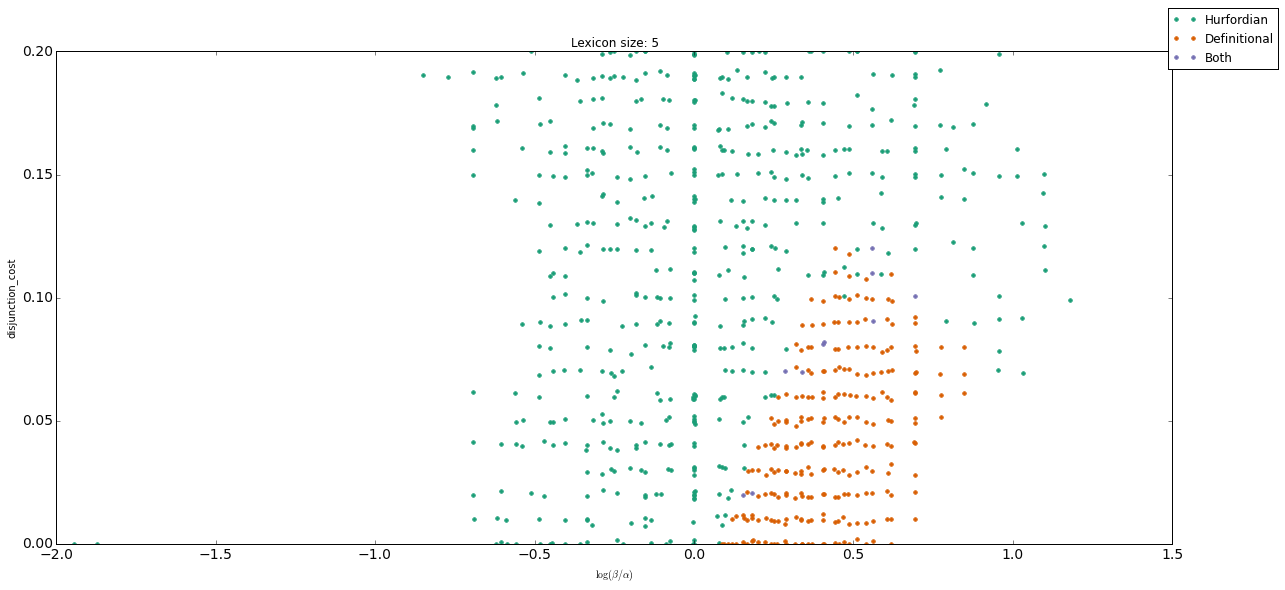
\includegraphics[width=1.2\textwidth]{fig/lex5-alpha-beta-gamma}

\end{examples}

%=====================================================================

\bibliographystyle{apalike}
\bibliography{levy-potts-pragdisj-bib}

\end{document}


